
\subsection{Appendix} \label{app: derivations}
\begin{figure} [H] 
    \centering
    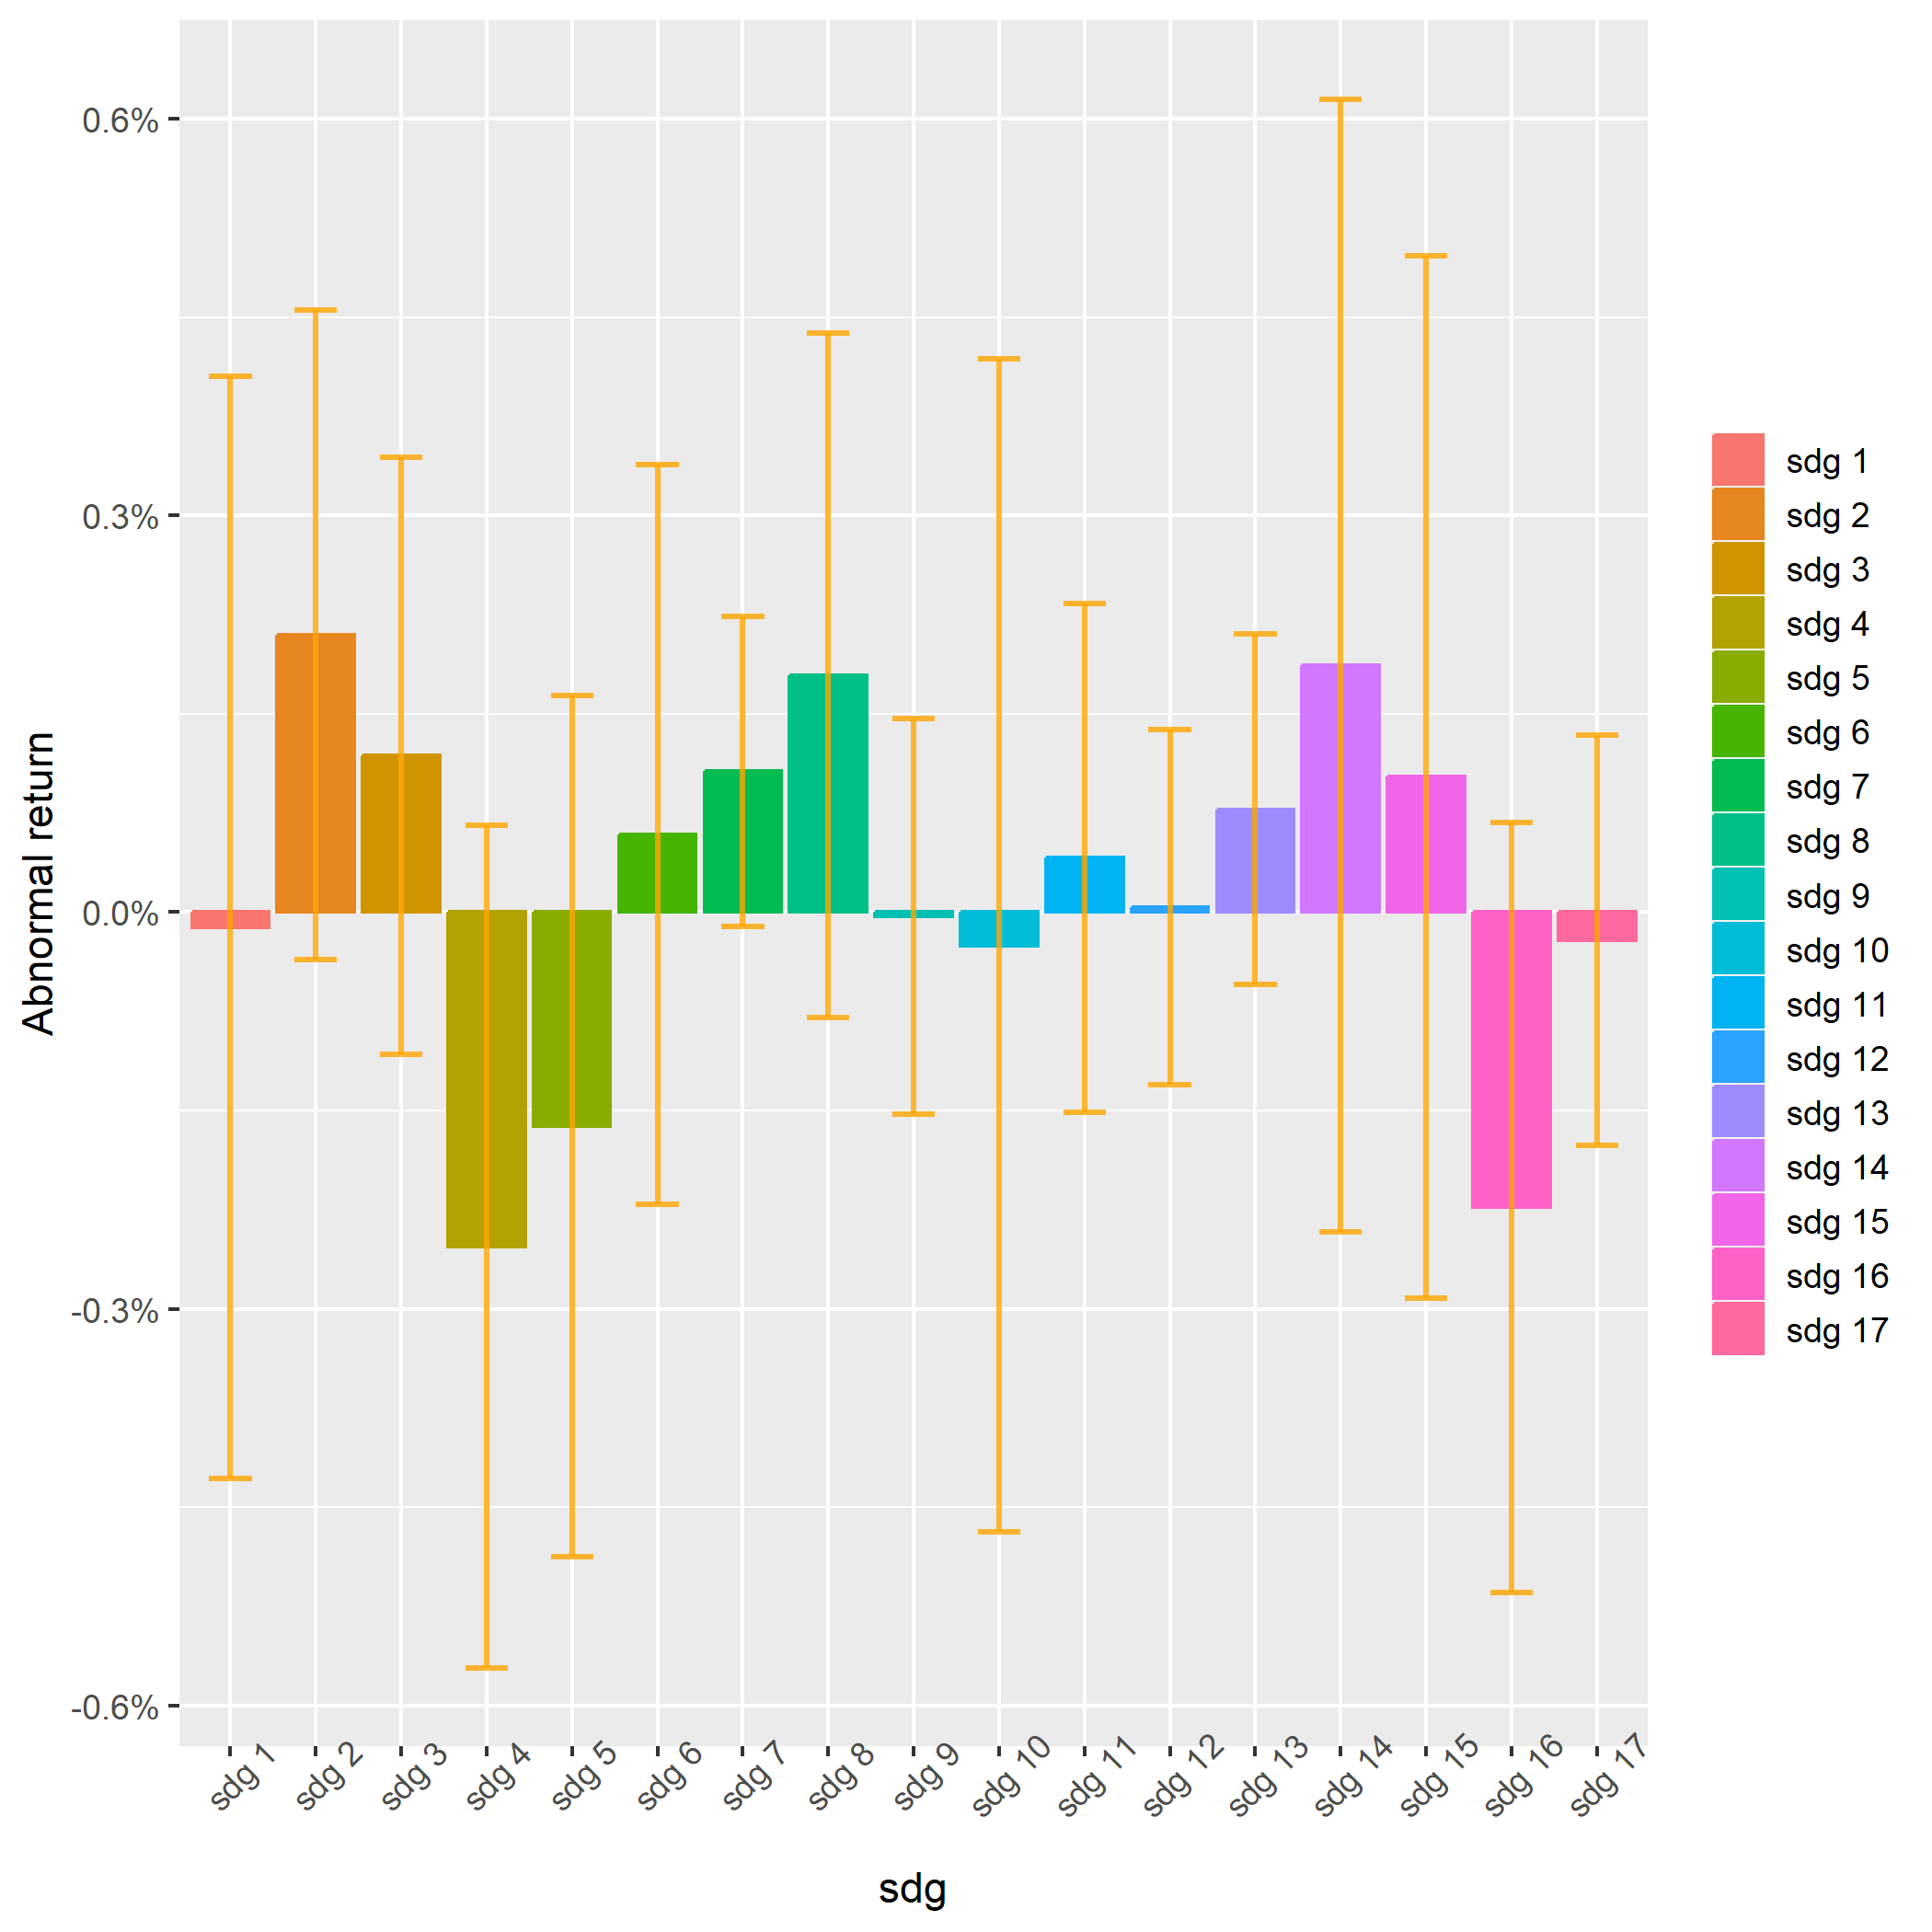
\includegraphics[scale=0.6]{Projekt/1.Figures analysis/ST_positive_sdg_bar_2.png} 
    \caption{Positive news split on SDG: $CAAR_{t=2}$}
    \label{fig:ST_pos_news}
\end{figure}

\subsection{Appendix} \label{app: derivations}
\begin{figure} [H] 
    \centering
    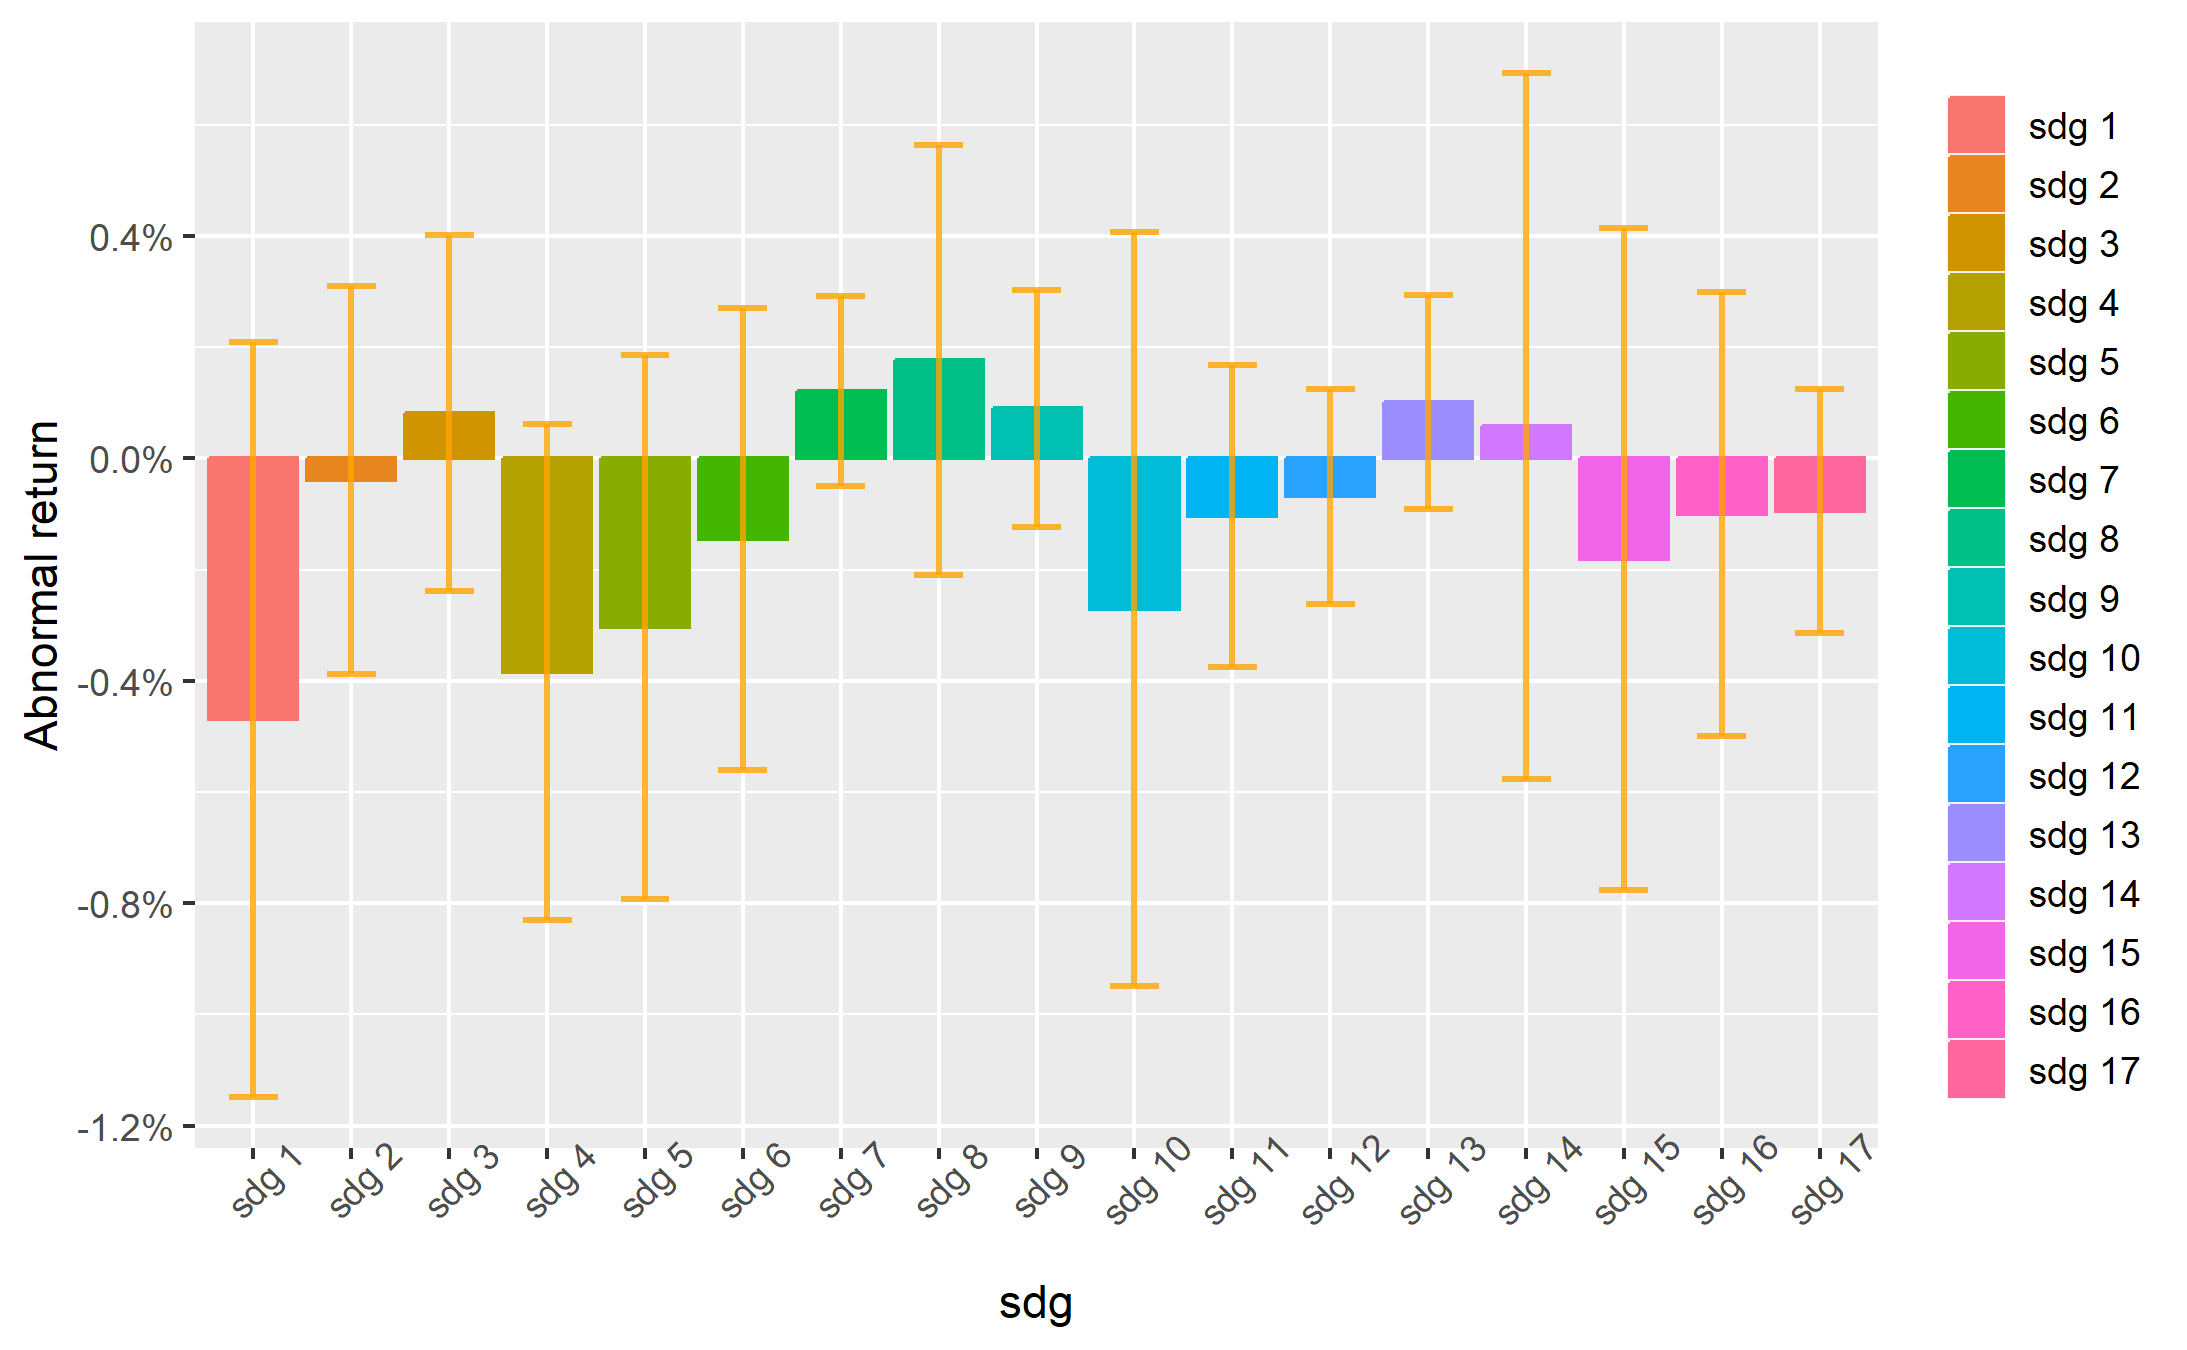
\includegraphics[scale=0.6]{Projekt/1.Figures analysis/ST_positive_sdg_bar_5.png} 
    \caption{Positive news split on SDG: $CAAR_{t=5}$}
    \label{fig:ST_pos_news}
\end{figure}

\subsection{Appendix} \label{app: derivations}
\begin{figure} [H] 
    \centering
    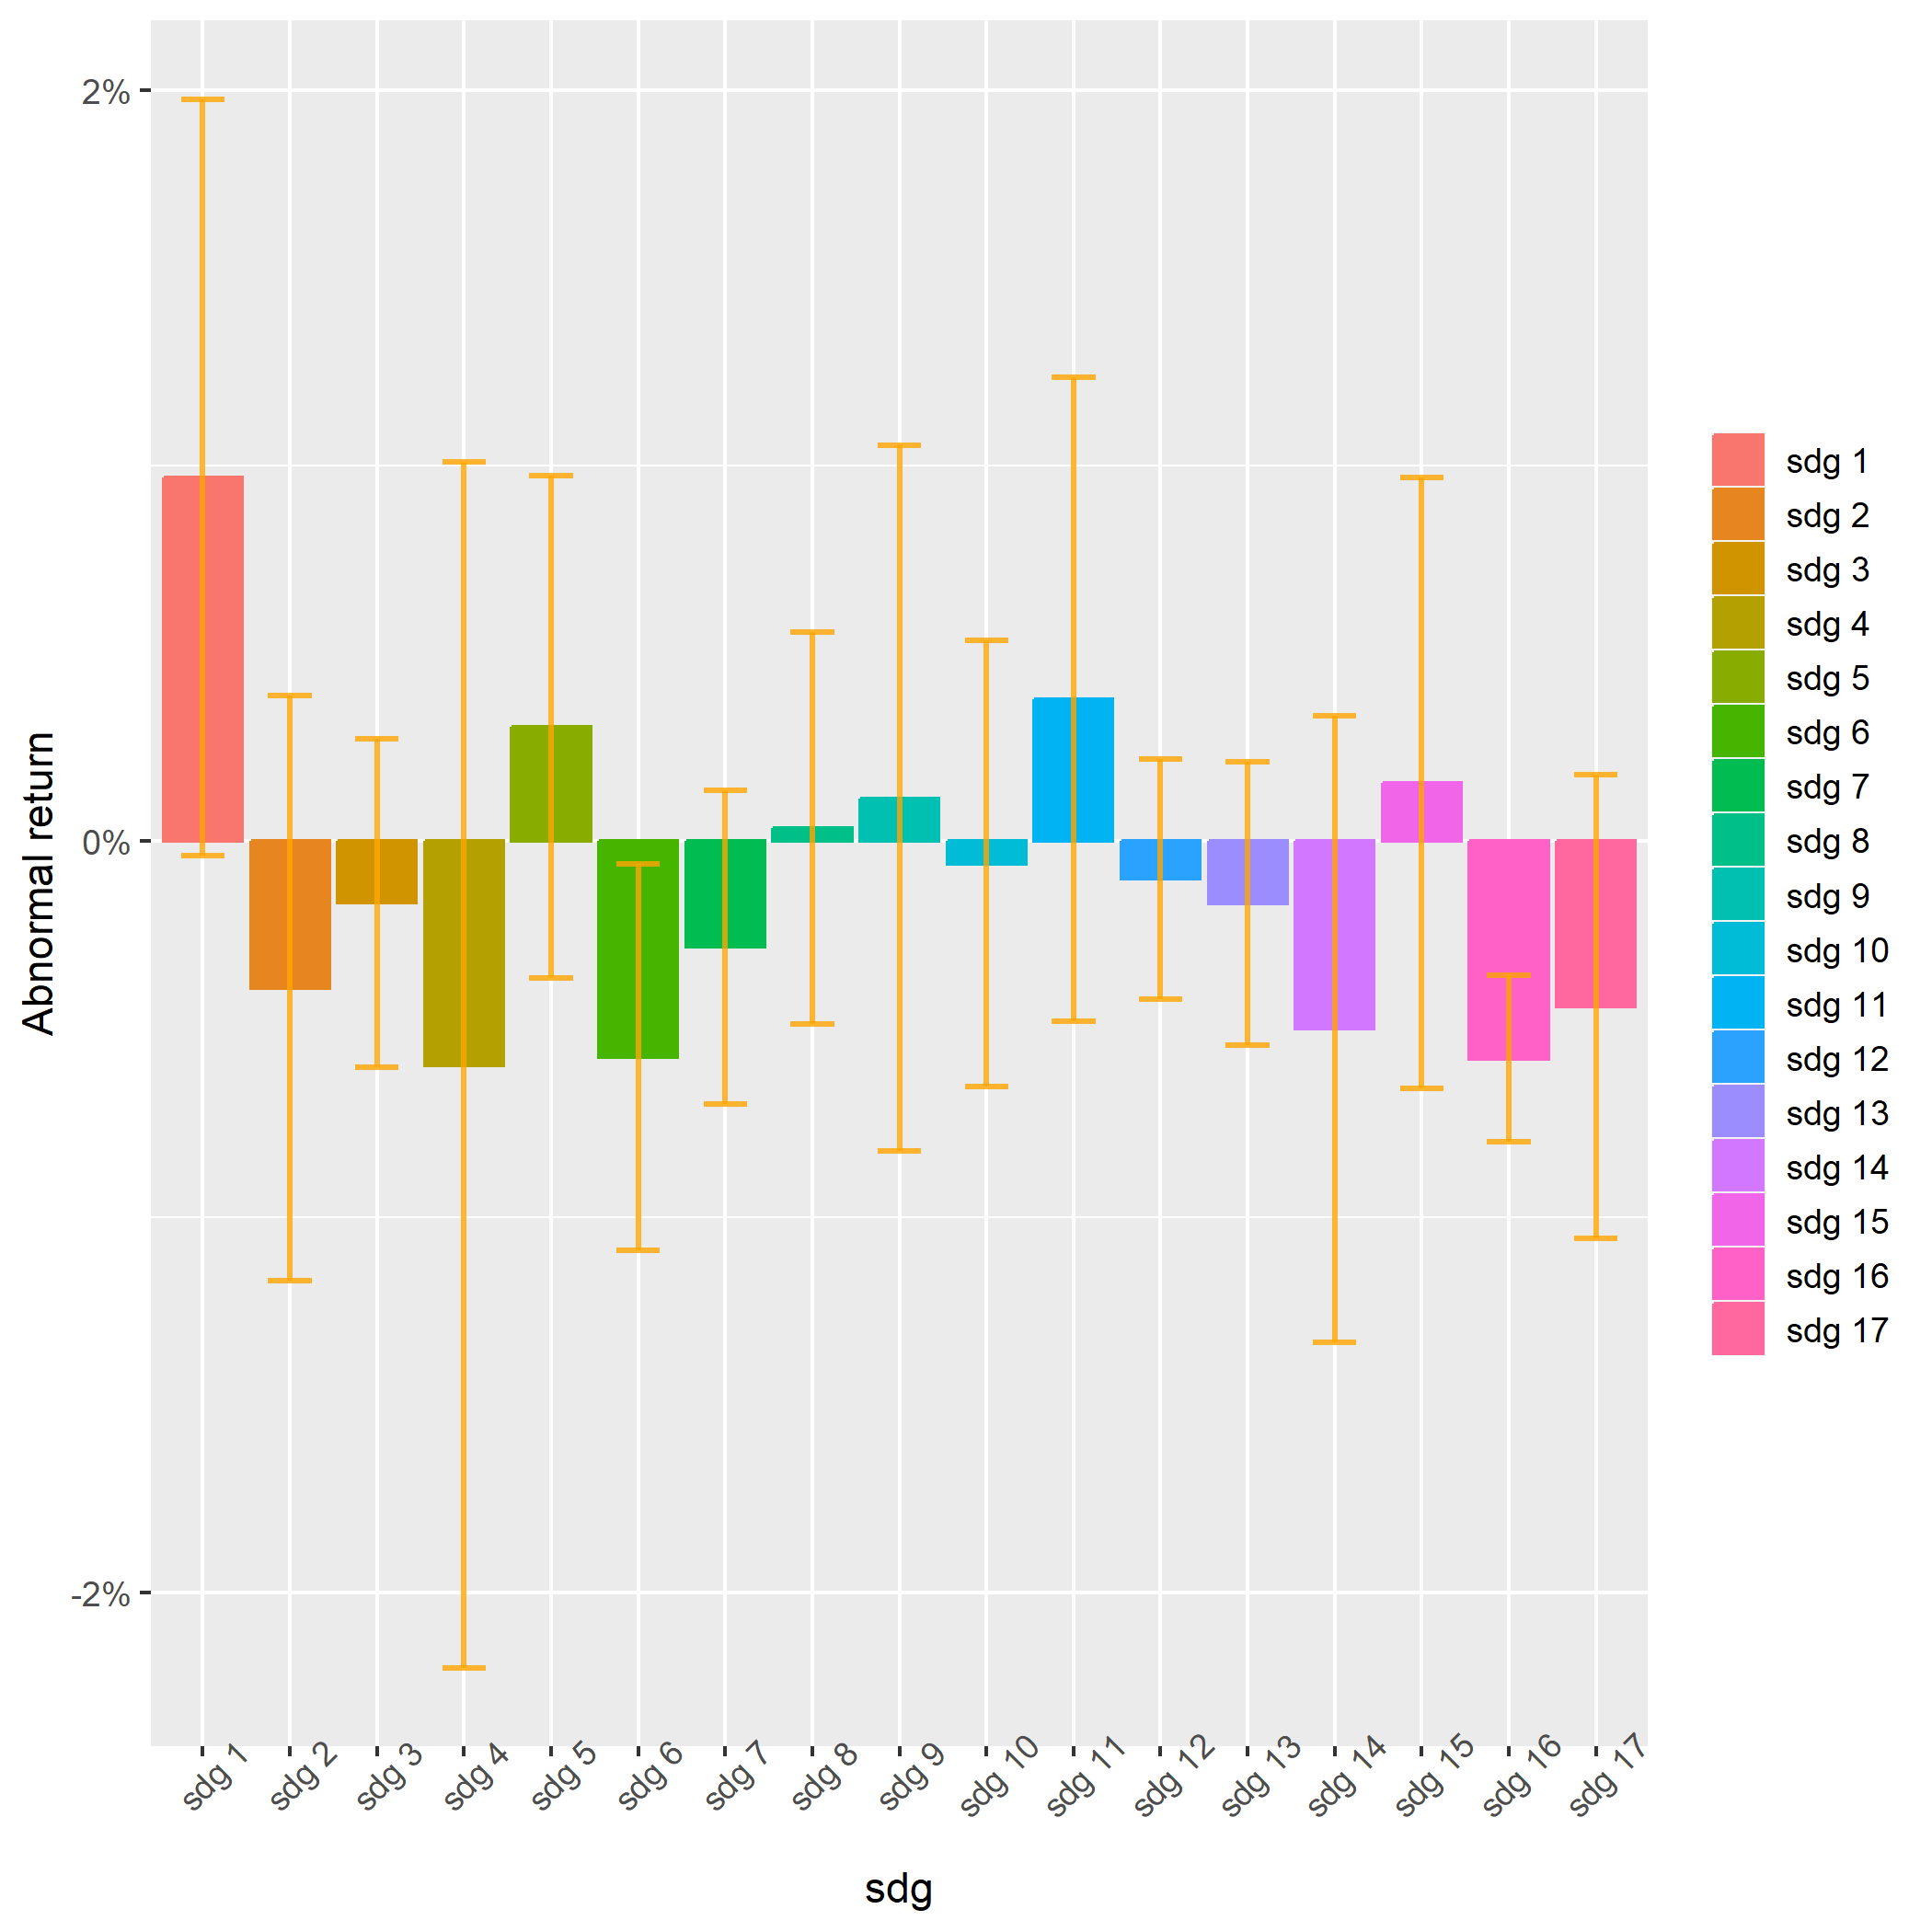
\includegraphics[scale=0.6]{Projekt/1.Figures analysis/ST_negative_sdg_bar_2.png} 
    \caption{Negative news split on SDG: $CAAR_{t=2}$}
    \label{fig:ST_pos_news}
\end{figure}

\subsection{Appendix} \label{app: derivations}
\begin{figure} [H] 
    \centering
    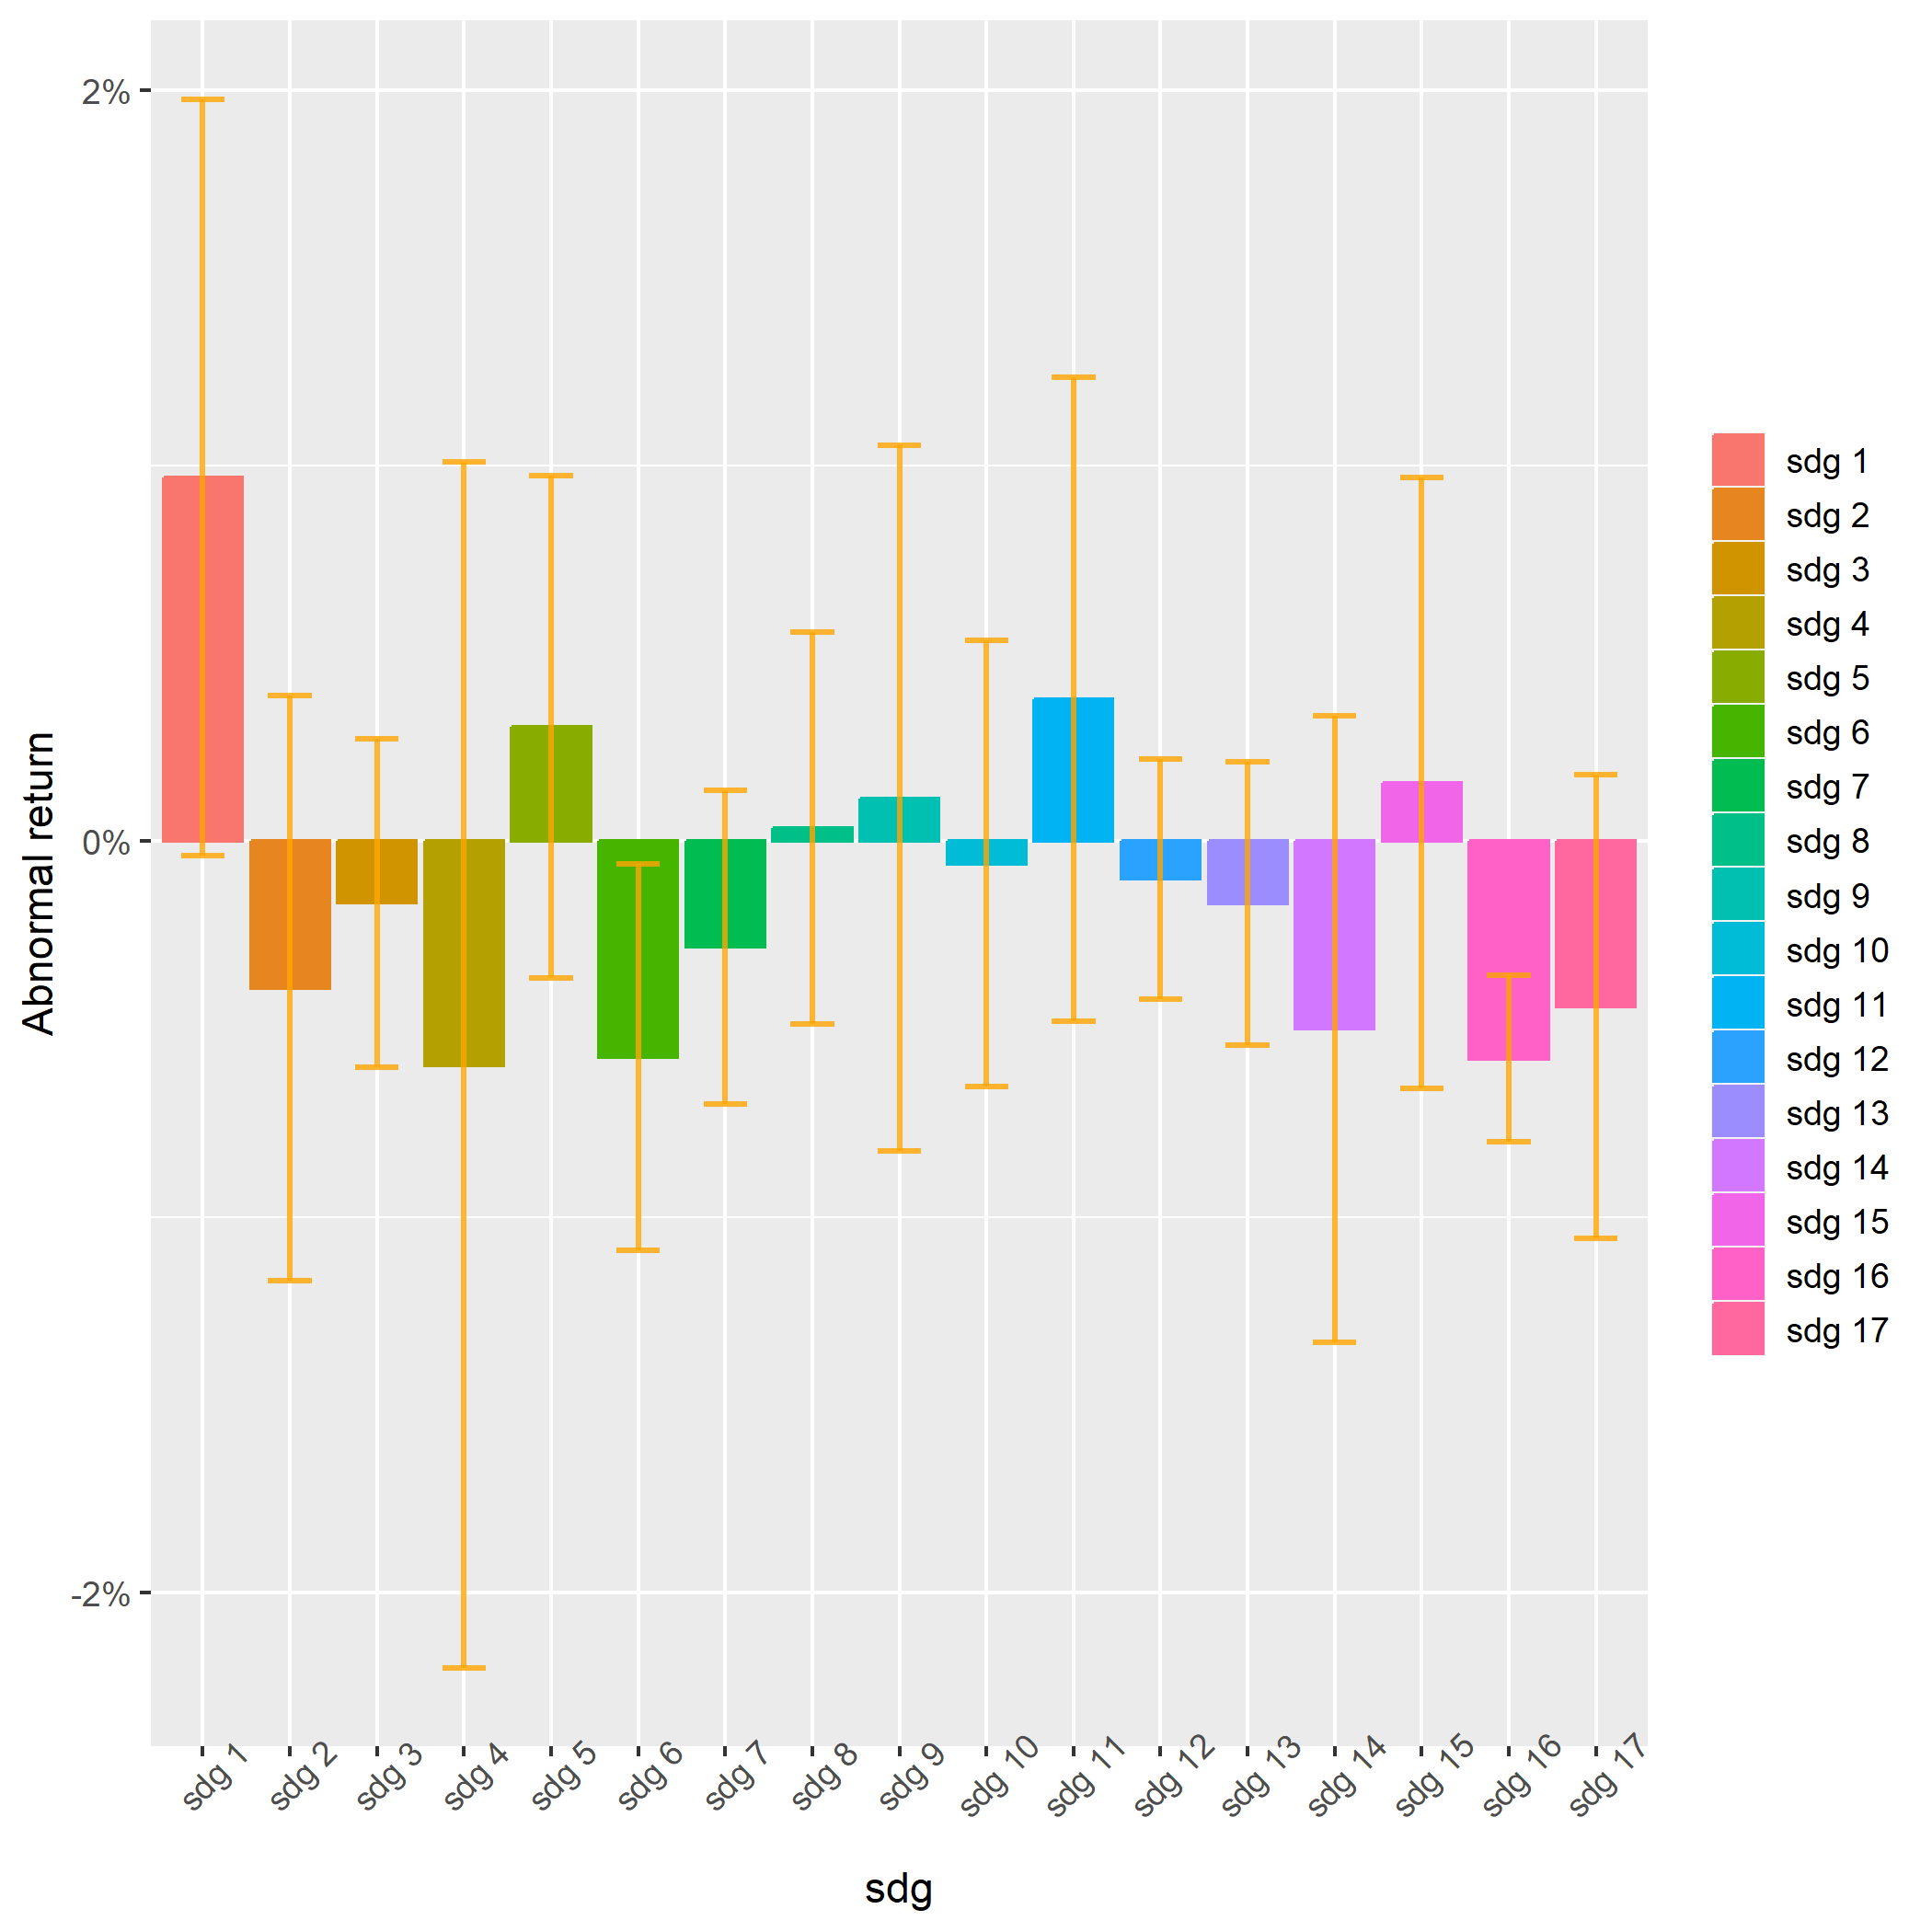
\includegraphics[scale=0.6]{Projekt/1.Figures analysis/ST_negative_sdg_bar_2.png} 
    \caption{Negative news split on SDG: $CAAR_{t=2}$}
    \label{fig:ST_pos_news}
\end{figure}


\begin{figure} [H]
    \centering
    \caption{Positive news: event identification rule}
    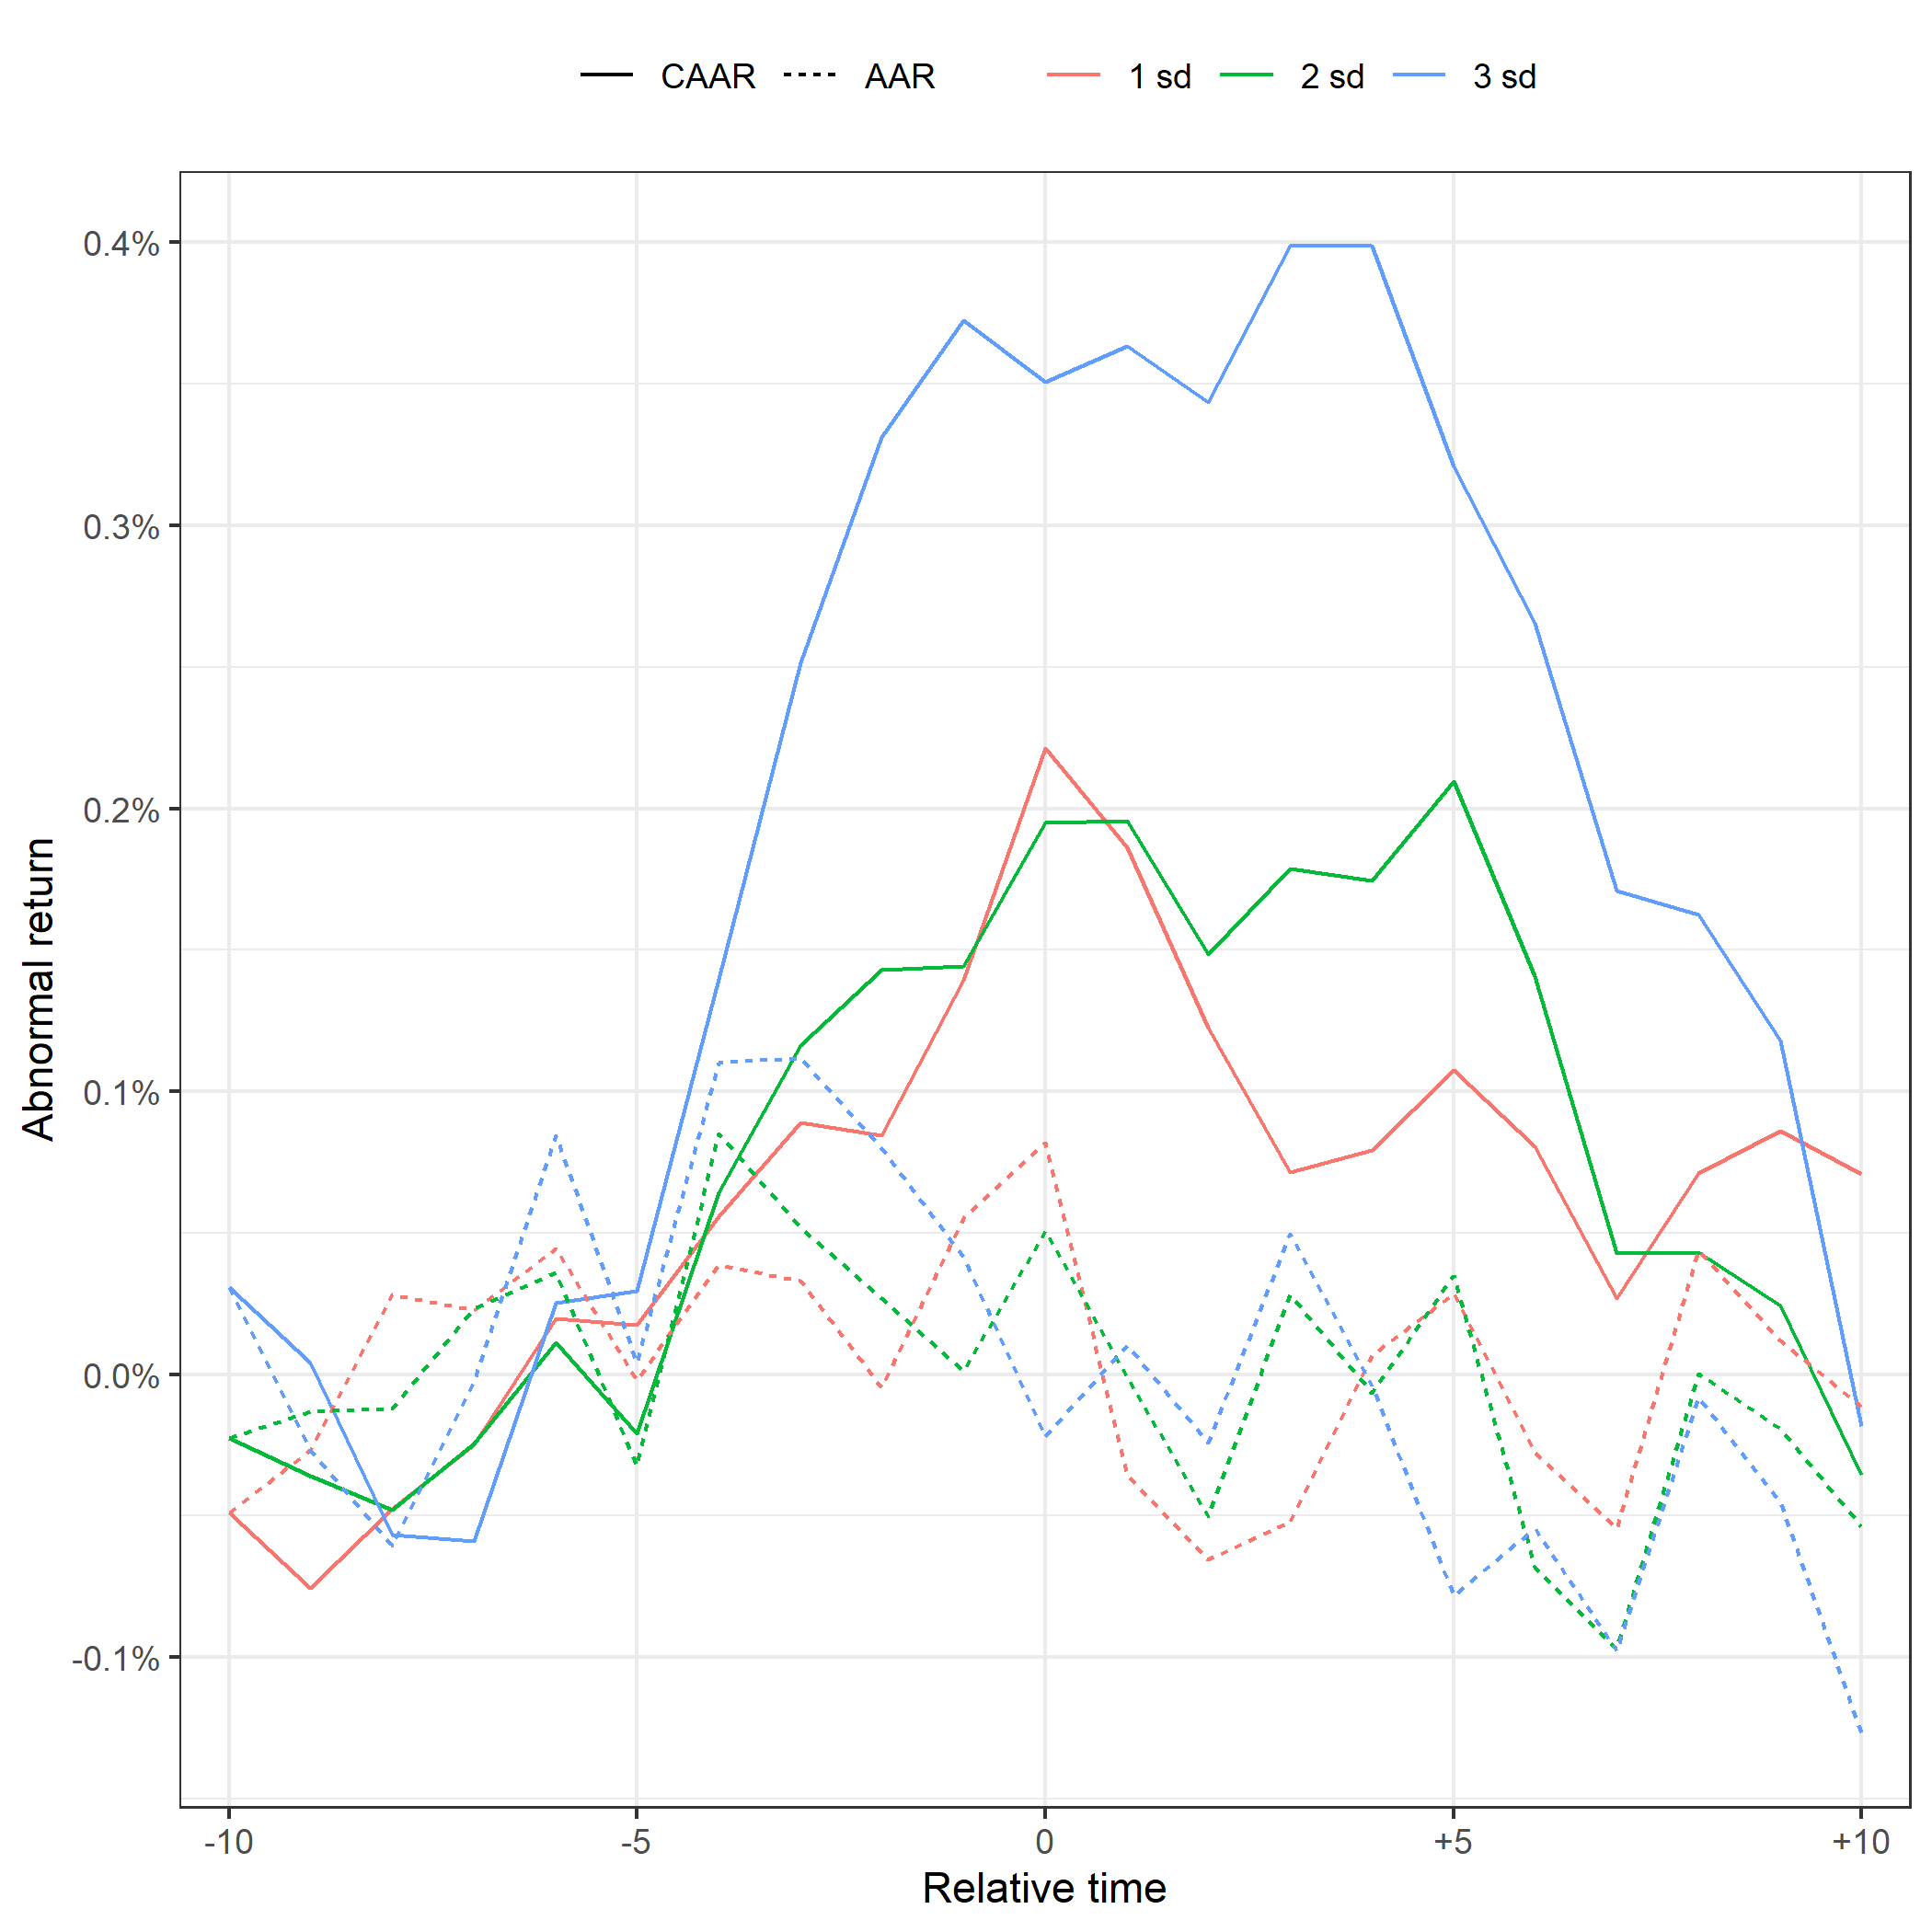
\includegraphics[scale=0.6]{Projekt/1.Figures analysis/ST_positive_sensitivity.png}
     \caption*{\footnotesize The figure illustrates the average abnormal return (AAR) and cumulative AAR (CAAR) around the event date (t = 0) of negative news. The figure illustrates the average abnormal return (AAR) and cumulative AAR (CAAR) around the event date (t = 0) of negative news. The various colors represent whether the event identification rule was based on 1, 2, or 3 standard errors. }
    \label{fig:ST_pos_sensi_sd}
\end{figure} 

\begin{figure} [H]
    \centering
    \caption{Positive news: Value vs. Equal weights}
    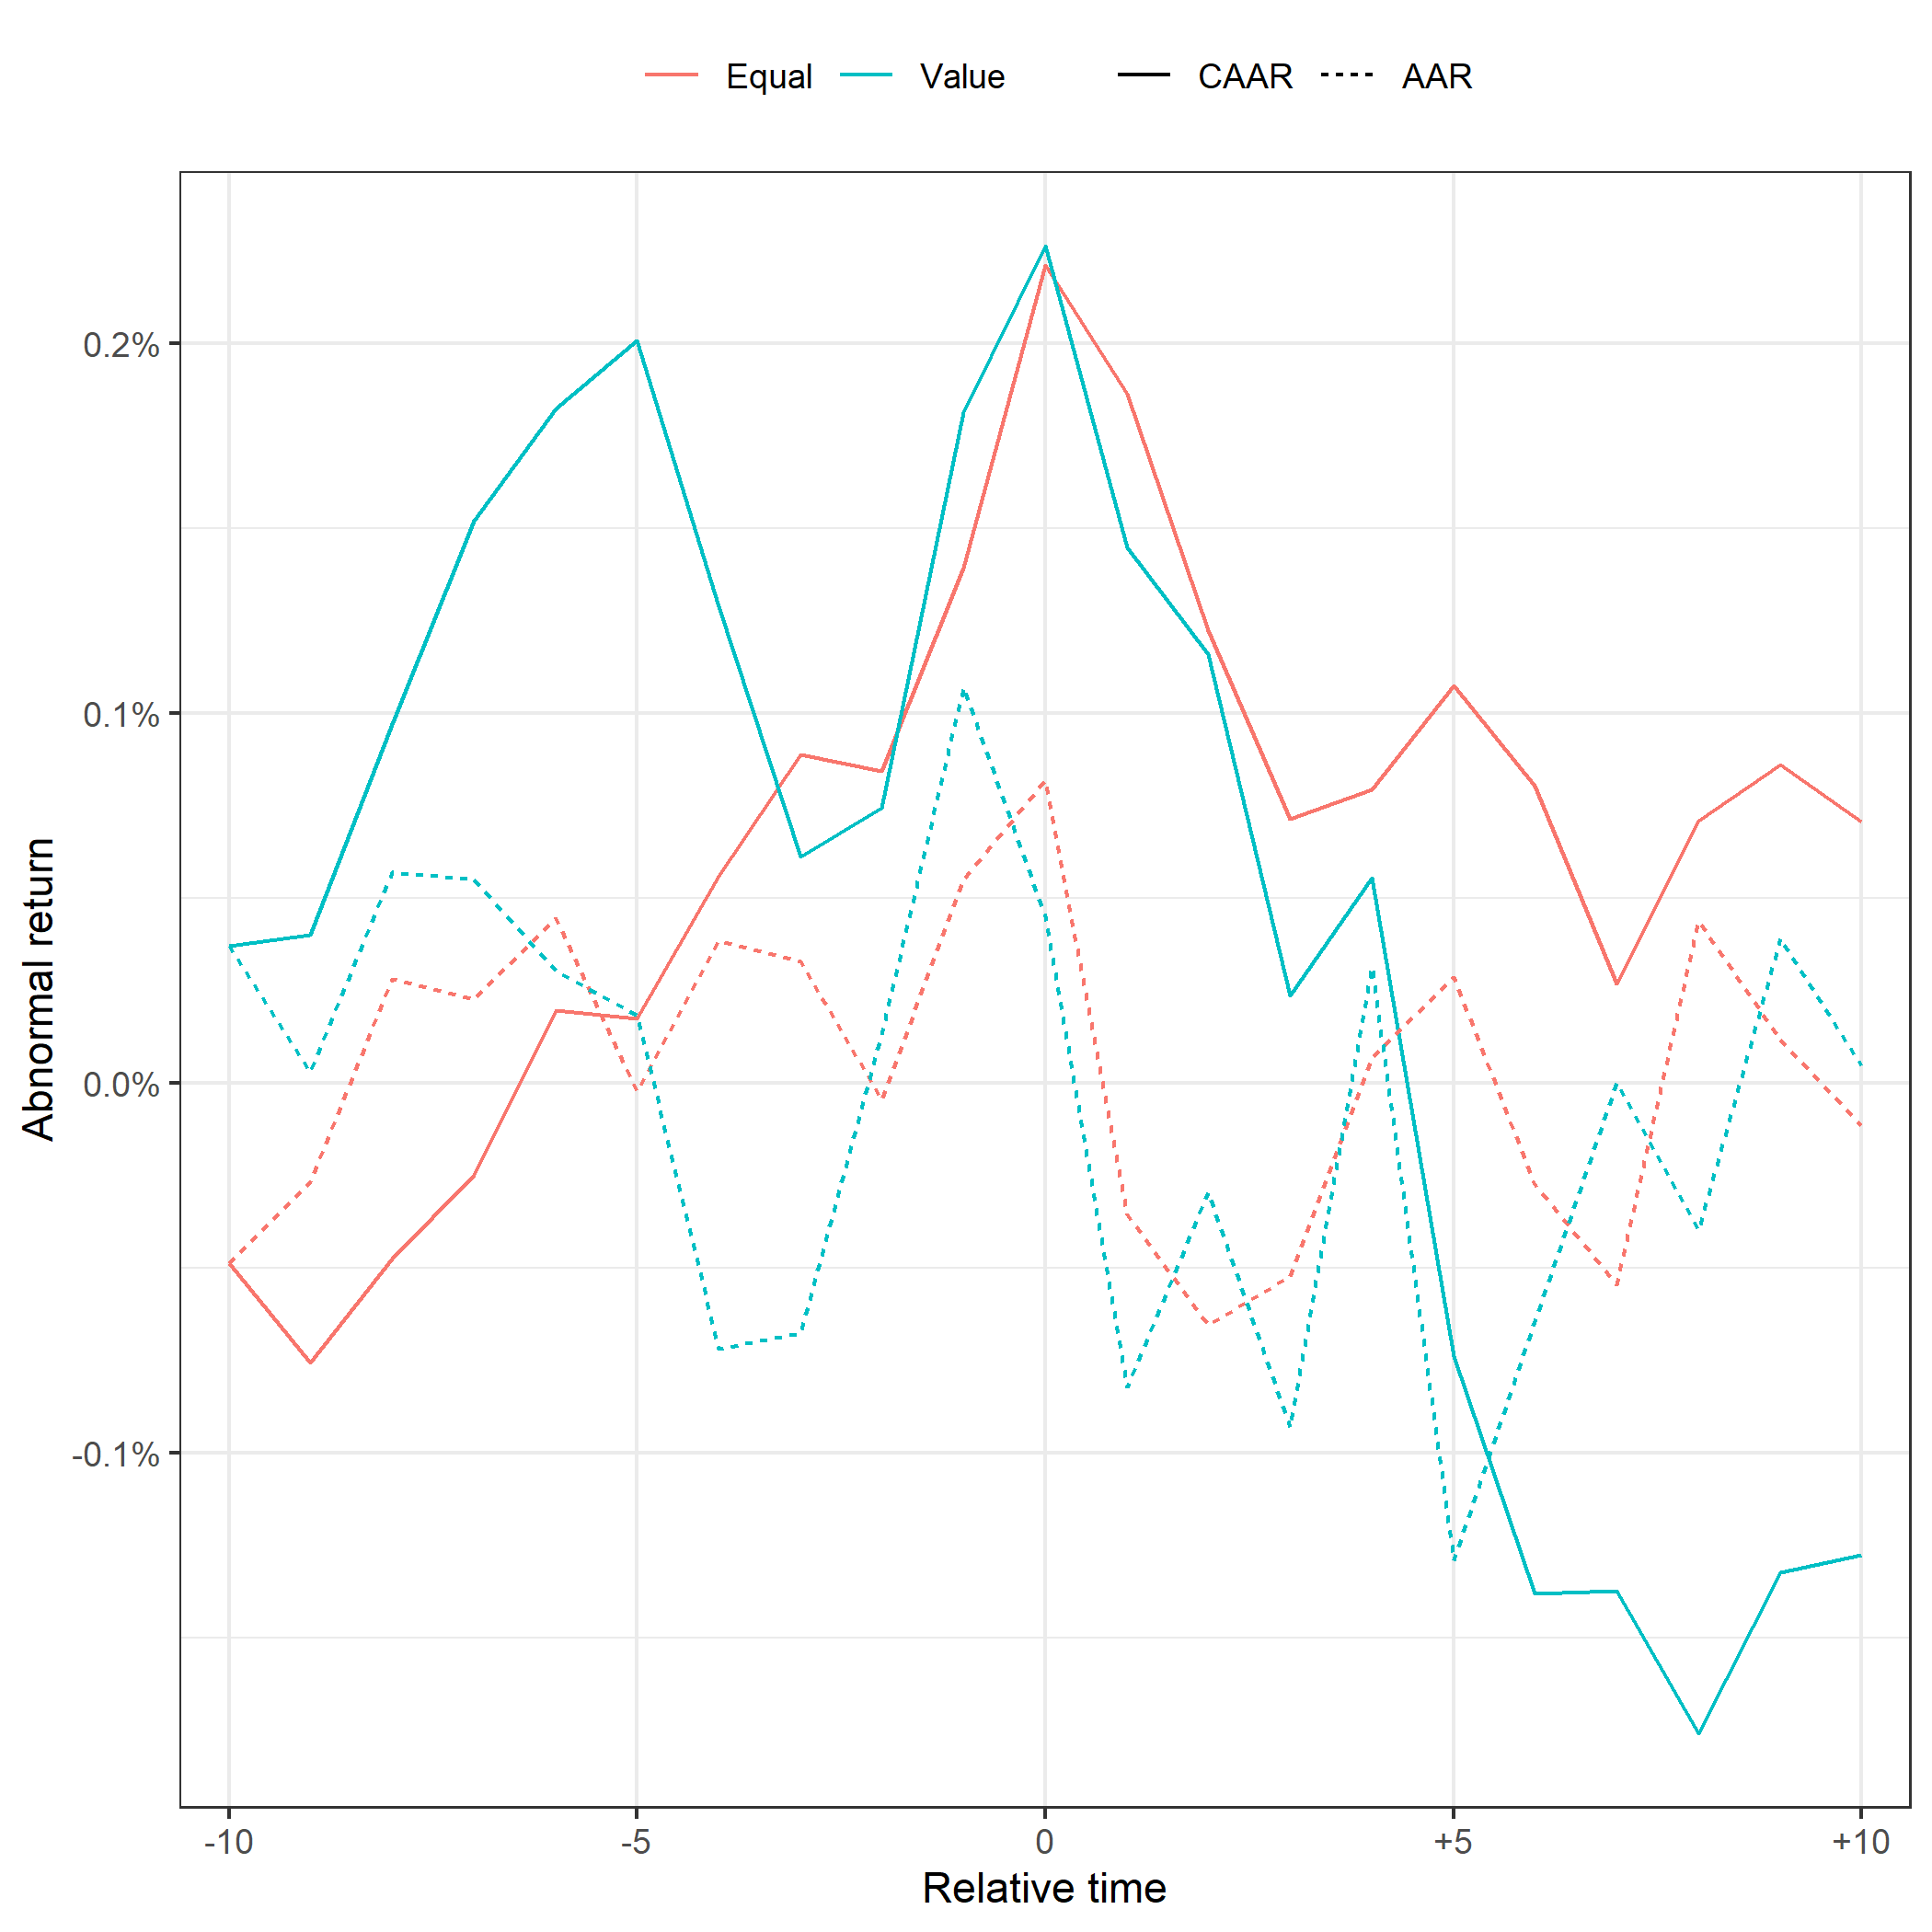
\includegraphics[scale=0.6]{Projekt/1.Figures analysis/ST_positive_sensitivity_weight.png}
     \caption*{\footnotesize The figure illustrates the average abnormal return (AAR) and cumulative AAR (CAAR) around the event date (t = 0) of positive news. The blue lines are returns calculated from an equally weighted portfolio, while the weights of the red lines are based on market capitalization. }
    \label{fig:ST_pos_sensitivity_weights}
\end{figure} 